\documentclass[english,11pt]{article}
\usepackage[T1]{fontenc}
\usepackage[utf8]{inputenc}
\usepackage{graphicx}
\usepackage{geometry}
\usepackage{caption}
\usepackage{subcaption}
\usepackage{babel}
\usepackage{amsmath}
\usepackage[nottoc,numbib]{tocbibind}
\usepackage{verbatim}
\usepackage{pdfpages}
\usepackage{hyperref}

\DeclareGraphicsExtensions{.png,.jpg}

\begin{document}

\title{Bioinformatics assessment 1 report}
\author{Motiejus Jakštys\\ 1003704}
\date{14 February 2013}

\maketitle
\tableofcontents

\section{Task 1}
\label{sec:task1}
See listing~\ref{lst:fgenesh}.

\section{Task 2}
What is interesting, during 1 week the search got a new feature which
I am sure wasn't there when I looked at the page last week. See
listing~\ref{img:blastp.png} for a screenshot. It shows putative conserved
domains which Blastp has found so far while the search is in progress.

\section{Task 3}
\texttt{ASZ1 protein [Homo sapiens]}. $100\%$ match.

\section{Task 4}
Since it is a $100\%$ match, getting the protein sequence for this protein would
be redundant. See the protein sequence in the end of listing~\ref{lst:fgenesh}.

\section{Task 5}
Like mentioned earlier in the report, it does not make sense to align two
identical proteins. They just match $100\%$.

\section{Task 6}
\label{sec:task6}
Most interesting number is bases masked. $53.73\%$. See more details in
listing~\ref{lst:repeatmasker}.

\section{Task 7}
Done.

\section{Task 8}
Chromosome 7. Detailed answer: \texttt{Homo sapiens BAC clone CTA-343P13 from
7 complete sequence}.

\section{Task 9}
\label{sec:task9}
During the lectures it was mentioned that we can use other exotic animal instead
of African elephant. I chose \texttt{Lemur catta}. However, unfortunately, I was
not able to find mRNA of neither \texttt{Lemur catta}, nor for the sequence I
was given.

\section{Task 10}
Just for clarification: I compared the protein of \texttt{Lemur catta}
(\href{http://www.ncbi.nlm.nih.gov/protein/AAY88997.1}{\texttt{AAY88997.1}}) with
protein acquired from masked sequence from section~\ref{sec:task6}.

\begin{description}
    \item[Score] 70.1 bits(170)
    \item[Expect] $10^{-16}$
    \item[Method] Compositional matrix adjust
    \item[Identities] $51/164$ ($31\%$)
    \item[Positives] $77/164$ ($46\%$)
    \item[Gaps] $9/164$ ($5\%$)
\end{description}

\section{Task 11}
Like mentioned in section~\ref{sec:task9}, I could not find these mRNA
sequences, so no comparison could be done.

\section{Task 12}
Initial sequence comparison gave $1852/2291$ ($81\%$) match, but with protein
sequence comparison it is only $46\%$. This is expected, because, like mentioned
in section~\ref{sec:task6}, there are over $53\%$ masked bases (repeats). That
means I was comparing only half of my initial sequence, and got roughly half the
match I got with nucleotides. Makes sense. It would be interesting to compare
masked human sequence with masked Lemur sequence. I expect to get $>80\%$ match
in that case.

\section{Listings}

\subsection{Figures}
\begin{figure}[h!]
    \centering
    \caption{Blastp during search}
    \label{img:blastp.png}
    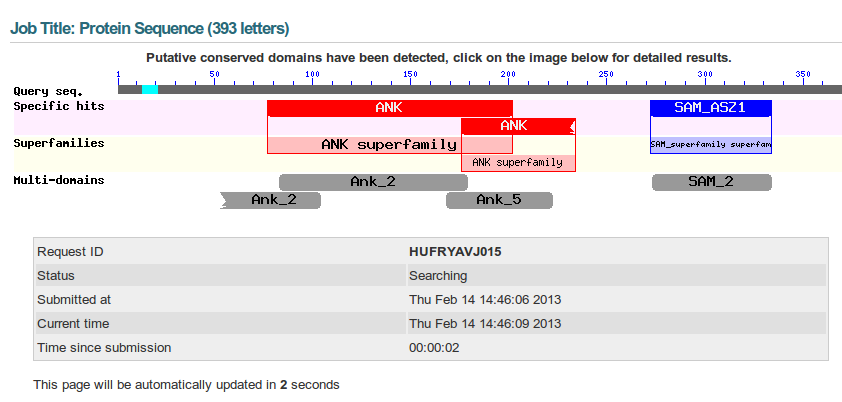
\includegraphics[width=0.8\textwidth]{blastp}
\end{figure}

\newpage

\subsection{Blastp search result}
\label{lst:fgenesh}
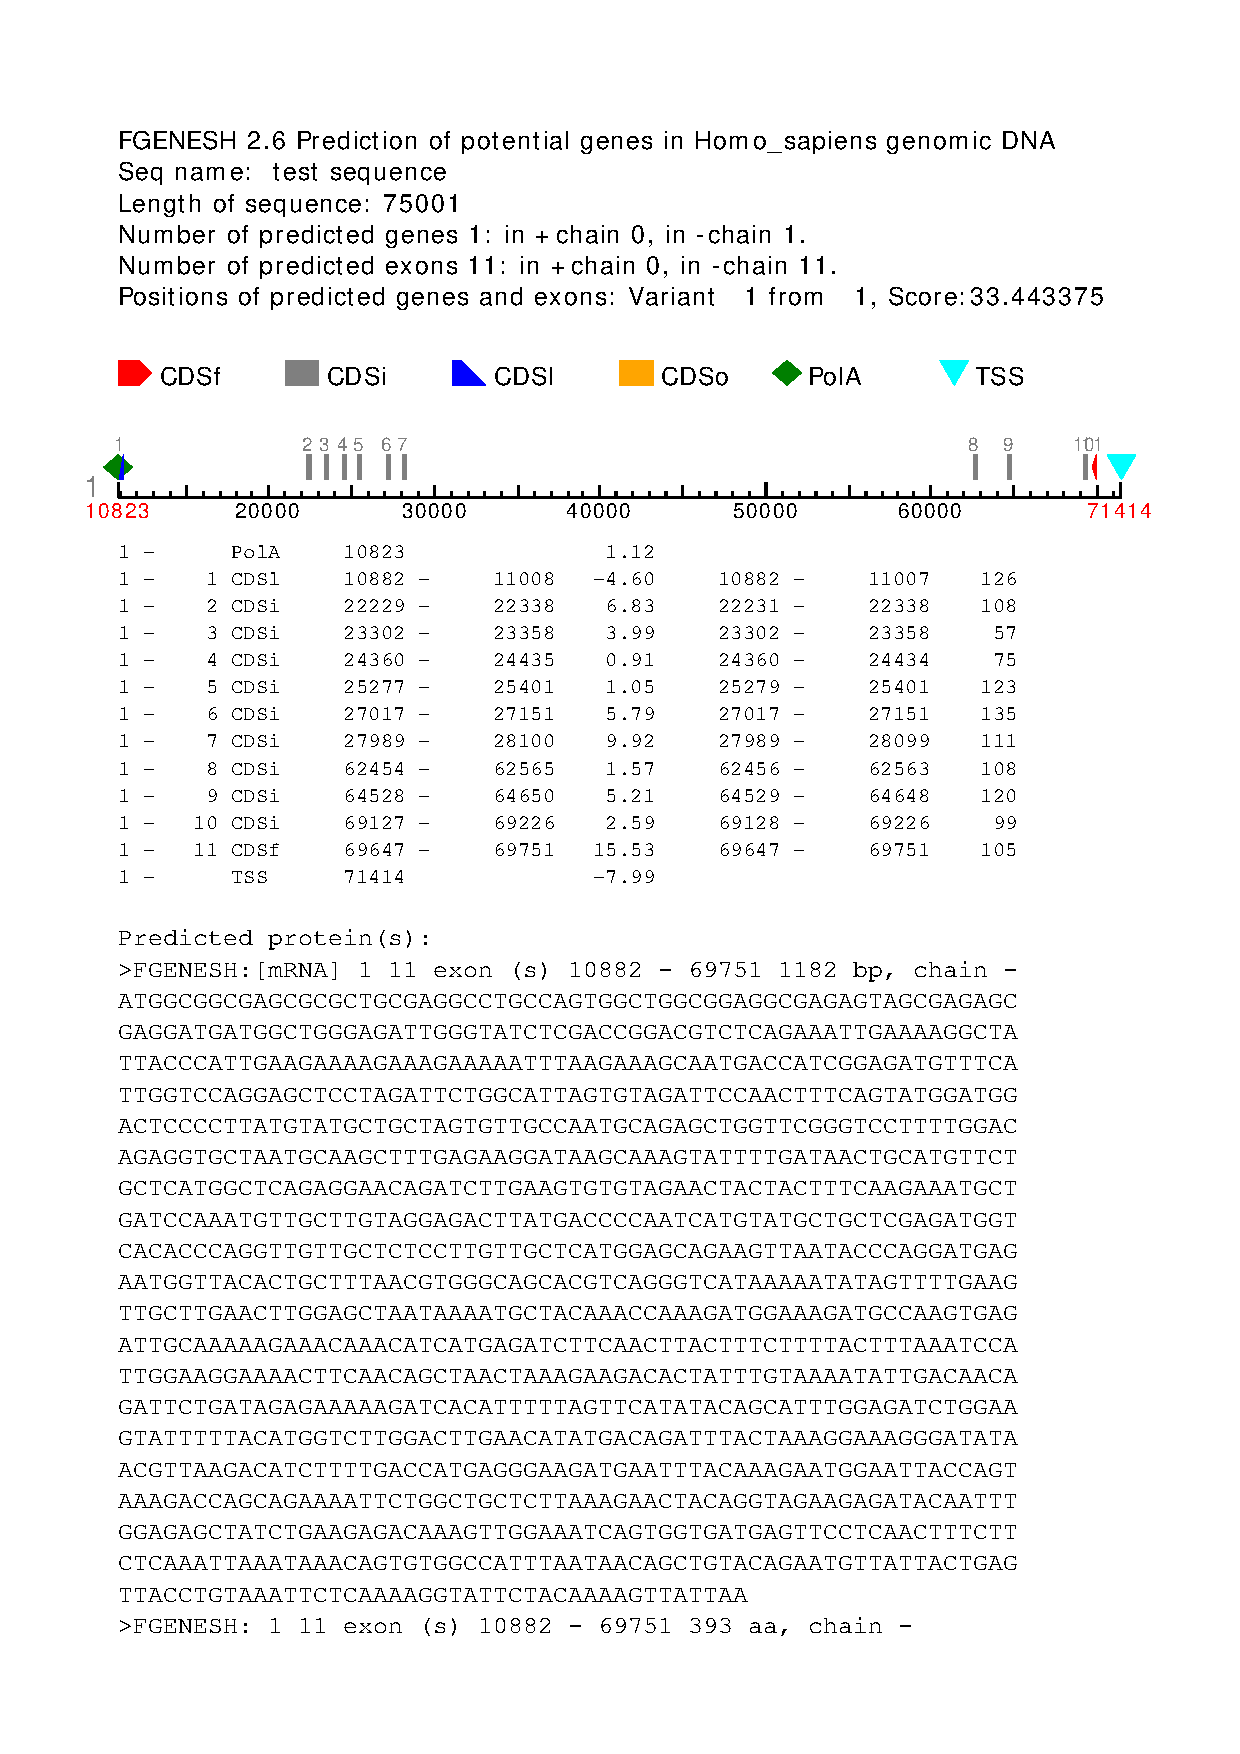
\includepdf[pages=-]{fgenesh.pdf}

\subsection{Repeat masker results}
\label{lst:repeatmasker}
{\small
    {\verbatiminput{repeatmasker.txt}}
}

\end{document}
